\documentclass{article}
\usepackage{fullpage}
\usepackage[czech]{babel}
\usepackage{amsfonts}
\usepackage{amsmath}
\usepackage{graphicx}
\usepackage{caption}
\usepackage{enumerate}
\graphicspath{{images/}}

\title{\vspace{-2cm}Fyzika druháku\vspace{-1.7cm}}
\date{}
\author{}

\begin{document}
\maketitle

\part{Struktura pevných látek}

\section{Krystalografické soustavy}
AAAAAAA

\section{Deformace}

  \begin{minipage}{0.25\textwidth}\raggedleft
    \begin{itemize}
      \item typy:
      \begin{itemize}
        \item tahem/tlakem
        \item kroucením
        \item ohybem
        \item smykem
      \end{itemize}
    \end{itemize}
  \end{minipage}
  \hspace{0.5cm}
  \noindent\begin{minipage}{0.12\textwidth}
    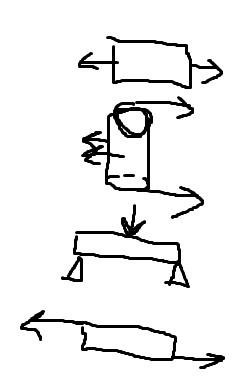
\includegraphics[width=0.9\linewidth]{deformace}
  \end{minipage}

  \section{Deformace tahem/tlakem}

    \begin{itemize}
      \item Normálové nápětí:
      	\begin{equation*}
          \sigma=F/S; [N/m^2] = [Pa]
        \end{equation*}
        \begin{center}
          \vspace{-0.25cm}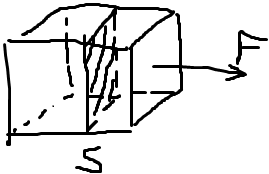
\includegraphics[width=0.12\textwidth]{normalove_napeti}\vspace{-0.25cm}
        \end{center}
      \item Změna délky:
        \begin{equation*}
          \Delta l = l - l_0; \ [m]
        \end{equation*}
      užitečnější většinou relativní prodloužení:
        \begin{equation*}
          \varepsilon = \Delta l/l_0; \ [bezrozm.]
        \end{equation*}
    \end{itemize}

    \subsection{Deformační křivka}
      \begin{center}
        \vspace{-0.1cm}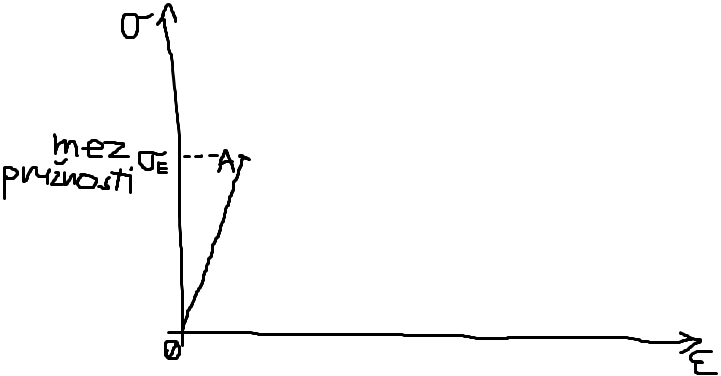
\includegraphics[width=0.75\linewidth]{deformacni_krivka}\vspace{-0.25cm}
      \end{center}

      \begin{itemize}
        \item lineární úsek (0 - A)
        \begin{itemize}
          \item pružná deformace
          \item vratná
          \item platí Hookův zákon:
            \begin{equation*}
              \varepsilon \propto \sigma
            \end{equation*}
          tedy slovy: relativní prodloužení je přímo úměrné napětí (ano, to je symbol pro přímou úměrnost, zapamatujte si ho)
            \begin{equation*}
              \sigma = E\cdot\varepsilon
            \end{equation*}
          E - Youngův modul pružnosti (např. ocel = 220 GPa, cín = 55 GPa, tj. tlak potřebný, abychom objekt roztáhli na dvojnásobnou délku)
        \end{itemize}
        \item nelineární deformace (A - B)
        \begin{itemize}
          \item plastická deformace
          \item protažení bylo dost velké, aby přesunulo atomy v krystalické mřížce na jiné místo
          \item materiál tedy ztráci schopnost se po deformaci vrátit do původního tvaru
          \item při překročení meze pevnosti se materiál prostě trhá na dva kusy
        \end{itemize}
      \end{itemize}

        \subsubsection{Příklady}
        \begin{enumerate}
          \item O kolik se protáhne ocelový drát když na něj zavěsíme závaží:
          \begin{equation*}
            d = 1 mm;
            l = 5 m;
            m = 30 kg;
            E = 220 GPa
          \end{equation*}
          \begin{itemize}
            \item[]
          \end{itemize}
          \begin{equation*}
            \sigma=\frac{F}{S}=\frac{300}{\pi\cdot0,0005^2}
          \end{equation*}
          \begin{equation*}
            \varepsilon = \frac{\sigma}{E}
          \end{equation*}
          \begin{equation*}
            \varepsilon = \frac{F}{S\cdot E}=\frac{\Delta l}{l_0}
          \end{equation*}
          \begin{equation*}
            \Delta l = \frac{F\cdot l\cdot 0}{S\cdot E}=8,7\cdot 10^{-3} m = 8,7 mm
          \end{equation*}
          \item Na ocelové lanko zavěsíme závaží. Jak těžké může být, aby se lanko nepřetrhlo:
          \begin{equation*}
            d = 1 mm;
            \sigma_p = 1,3 GPa;
            K = 5
          \end{equation*}
          \begin{enumerate}
            \item závaží je v klidu
            \item závaží se hýbe nahoru
            \begin{equation*}
              a = 1 m/s^2
            \end{equation*}
            \item jako kyvadlo OBRAZEKOBRAZEK
          \end{enumerate}
        \end{enumerate}

\part{Změny skupenství}
Př.: OBRAZEKOBRAZEK
$m = 0,2 kg$
a) teplota varu: 50 stupnu
b) c(kap.) $c = Q(m\cdot \Delta t)=200/(0,2 \cdot 40) = 25$ $Jkg^{-1}K^{-1}$
c) c(plyn) $c = Q(m\cdot \Delta t)=200/(0,2 \cdot 20) = 50$ $Jkg^{-1}K^{-1}$
d)$L_v$ -- skupenské teplo varu [J]
$L_v = 300 J$
$l_v = $ měrné skupenské teplo varu $l_v = L_v/m$ $[Jkg^{-1}]$
$l_v = 300/0,2 = 1500 Jkg^{-1}$

Pozn.: pro vodu: $l_t$ (tání) $= 332 Jkg^{-1}$
$l_v = 2257 Jkg^{-1}$

Př.: 1 kg vody z teploty -20 stupnu -> pára 100 stupnu, $P = 1 kW$
led -20 stupnu -> led 0 stupnu: ($c_{ledu} = 2100 Jkg^{-1}$) $Q = m\cdot c\cdot \Delta t = 42 kJ$ -> 42 s
led 0 stupnu -> voda 0 stupnu: $L_t = m\cdot l_t = 332 kJ$ -> 5 min 32 s
voda 0 stupnu -> voda 100 stupnu ($c_{vody} = 4180 Jkg^{-1}$) $Q = m\cdot c \cdot \Delta t = 418 kJ$ -> 6 min 58 s
voda 100 stupnu -> pára 100 stupnu: $L_v = m\cdot l_v = 2257 kJ$ -> 37 min 37 s (to je šílený)

Pozn.: Hranaty graf plati u krystalickych latek, u amorfnich latek (kvuli nedokonalostem v uskupeni) je graf obly OBRAZEKOBRAZEK
AAAAAAAAA REALNE TOHLE NEMAM SANCI DODELAT

\part{Kmitání}
Oscilátor: cokoliv co kmitá, např. kyvadlo, pravítko (lol)

\section{Kinematika oscilátoru}
Zjednodušení: uvažujeme tzv. harmonický oscilátor -- nemá ztráty, kmitá stále stejně (grafem je sinusoida)
Značení: $y$ -- okamžitá výchylka
         $y_m$ -- maximální výchylka (max. amplituda), y je z [$-y_m$;$y_m$] AAAAAAA
         T -- perioda [s]
         f -- frekvence [$s^{-1}$=Hz], $f\cdot T=1$
        $\omega$ -- úhlová frekvence (ekviv. úhlová rychlost), $\omega=\frac{\alpha}{t}=\frac{2\pi}{T}=2\pi f [s^{-1}]$
        v -- obvodová rychlost, $v=\frac{s}{t}=\frac{2\pi r}{T}=2\pi rf [ms^{-1}]$
Pozn.: Průmět přímoč. pohybu po kružnici na jedné ose je sinusoida -- kmitání je točení v jedné ose
Poloha: OBRAZEKOBRAZEK $y=y_m\cdot \sin(\alpha)$, přejmenujeme $\rightarrow y_m$, $\alpha = \omega t \Rightarrow y=y_m\cdot \sin(\omega t)$, popř. $y=y_m\cdot \sin(\omega t+{\phi}_0)$, ${\phi}_0$ -- počáteční fáze (případný offset na začátku od nul. úhlu)
Př.: pružinový oscilátor: $y_m=10cm$, $T=1,2s$
        a) rovnice: $\omega = \frac{2\pi}{T}=\frac{5\pi}{3}s^{-1}$
                    $y=0,1\cdot \sin(\frac{5\pi t}{3})$
        b) poloha v čase t=0,5 s: $y=0,1\cdot \sin(\frac{5\pi t}{6})$ POZOR RAD!!!
                                  $y=5cm$
Př.: Rychlost oscilátoru
     $\cos (\alpha) = v/v_0$
     $v=v_0\cdot \cos (\alpha)$
        1) $\alpha = \omega \cdot t$
        2) $v_0 = \omega \cdot r$
        3) $r = y_m$
     $\Rightarrow v = \omega \cdot y_m \cdot \cos(\omega t + {\phi}_0)$
     $v = \frac{2 \pi}{1,1}\cdot \cos(t)$

Zrychlení: OBRAZEKOBRAZEK
           $v_1 = \omega \cdot r$
           $a_d = \frac{{v_1}^2}{r} = \omega^2 \cdot r = \omega^2 \cdot y_m$

           $a = a_d \cdot sin(\omega t + {\phi}_0)$
           $a = \omega^2 \cdot y_m \cdot sin(\omega t + {\phi}_0) = \omega^2 \cdot y$ $\Rightarrow$ velikost zrychlení je přímo úměrná okamžité odchylce
           $a_{max} = \omega^2 \cdot y_m$

AAAAAAA hrozně moc pomooc

Př.: Závisí tuhost pružiny na počtu závitů
     ANO, k {vlnovka} $\frac{1}{n}$
     AAAAAA progresivní pružina (damn liberals)

\subsection{Fyzikální kyvadlo}
\begin{itemize}
  \item cokoliv zavěšeného mimo těžiště, tj. v rovnovážné poloze nad těžištěm
  \item mám těleso, jeho těžiště T, osu otáčení o a délku d mezi nimil
\end{itemize}

\section{Tlumené kmitání}
\begin{itemize}
  \item kromě síly, která je $F \propto -y$ působí i odporová síla, $F_{ODP} \propto -v, F_{ODP} \propto -b\cdot v$; b -- součinitel linearního odporu [$kg/s$] OBRAZEKOBRAZEK
  \item $y = y_m \cdot e^{- \frac{bt}{2m}}\cdot \sin(\omega' t + {\phi}_{0})$
  \item důsledky
  \begin{enumerate}
    \item je-li b malé ($b^2 << 4mk$); AAAA Př.: tlumí se to velmi pomalu
    \item Je-li b velké ($b^2 > 4mk$), kmitání je ztlumeno tak moc, že ani nekmitá, nemá to dost velkou sílu -- $\omega$ = sqrt{záporné číslo} OBRAZEKOBRAZEK
  \end{enumerate}
\end{itemize}

\section{Energie pružinového oscilátoru}
\begin{itemize}
  \item kinetická: $E_k = \frac{1}{2}mv^2=\frac{1}{2}m\cdot{y_m}^2\cdot\omega^2\cdot \cos^2(\omega t)=\frac{1}{2}k\cdot{y_m}^2\cdot \cos^2(\omega t)$
  \item $cos(2x)=2 \cos^2(x)-1$; $\cos^2(x) = \frac{1+cos(2x)}{2}$ OBRAZEKOBRAZEK y a Ek
  \item potenciální: $E_p = W = \frac{1}{2}F\cdot y$
\end{itemize}

\section{Vlnění}
\begin{itemize}
  \item $y(x, t) = y_m \sin\left(\frac{2\pi}{\lambda} x - 2\pi f t + \phi\right)$
\end{itemize}

\subsection{Interference vlnění}
\begin{itemize}
  \item skládání vlnění, když se vlny potkají, tak se jednoduše sečtou $y = y_1 + y_2$ OBRAZEKOBRAZEK
  \item pro jednoduchost budeme skládat vlnění se stejnou $\lambda$, f a s různou fází
  \item vlny můžeme jednoduše sčítat pomocí fázorů a kosinové věty
  \item speciální případy
  \begin{itemize}
    \item fázory jsou identické -- konstruktivní interference, dvakrát větší amplituda, stejná frekvence, vln. délka
    \item fázory jsou protilehlé -- destruktivní interference, nulová amplituda
  \end{itemize}
\end{itemize}

\subsection{Stojaté vlnění}
\begin{itemize}
  \item interference postupné a odražené vlny
  \item $y_1 = y_m sin(\omega t - kx)$
  \item $y_2 = y_m sin(\omega t + kx)$
  \item $y = y_1 + y_2 = y_m(sin(\omega t - kx)+sin(\omega t + kx)) = 2y_m cos(kx)sin(\omega t) = Y_m sin(\omega t)$ OBRAZEKOBRAZEK
  \item najdeme tady uzly (vždy 0, čili cos(kx)=0 čili v každém lichém násobku $\frac{\pi}{2}$) a kmitny (kmitají nejvíc, čili cos(kx)=max. čili v každém násobku $\pi$)
  \item odraz vlnění
  \begin{itemize}
    \item pevný konec: po odrazu se otočí fáze, interferují tedy destruktivně a pevný konec je uzel (logicky)
    \item volný konec: neotáčí se fáze, vznikne tedy kmitna
  \end{itemize}
  \item Př.: stojaté vlnění na struně g
\end{itemize}

\part{Elektrostatika}
\begin{itemize}
  \item eletkrický náboj -- Q [C -- Coulomb] (analogie hmotnosti)
\end{itemize}
\section{Elektrické pole}
\begin{itemize}
  \item intensita elektrického pole -- $\overrightarrow{E} = \frac{\overrightarrow{F_e}}{Q}$ [N/C]
  \item směr $\overrightarrow{E}$ = směr síly na kladný náboj OBRAZEKOBRAZEK
\end{itemize}
\subsection{Typy elektrického pole}
\subsubsection{Homogenní pole}
\begin{itemize}
  \item $\overrightarrow{E}$ = konst. OBRAZEKOBRAZEK
\end{itemize}
\subsubsection{Radiální pole}
\begin{itemize}
  \item E = $\frac{k\cdot\frac{Q_1 Q_2}{r^2}}{Q_2} = k\cdot\frac{Q_1}{r^2}$ OBRAZEKOBRAZEK
\end{itemize}
\subsubsection{Dipólové pole}
\begin{itemize}
  \item dva náboje opačného znaménka -- $Q_1 = Q_2$ OBRAZEKOBRAZEK
\end{itemize}
\subsection{Potenciál elektrického pole}
\begin{itemize}
  \item $\phi = \frac{E_p}{Q}$ [J/C]; $E_p$ -- potenciální energie
  \item ekvipotenciální plochy -- místa se stejným potenciálem -- vždy kolmé na siločary
\end{itemize}
\subsection{Práce, energie}
\begin{itemize}
  \item $W = F\cdot s = F\cdot s\cdot \cos \alpha $
\end{itemize}
\subsubsection{V homogenním poli}
\begin{itemize}
  \item $E = \frac{F}{Q} = konst.$
  \item $F = EQ$
  \item $W = E\cdot Q\cdot s = E\cdot Q\cdot s\cdot \cos \alpha = E\cdot Q\cdot d$; d je vzdálenost kolmá na siločary OBRAZEKOBRAZEK elektricka\_prace
  \item $W = \Delta E_p$
  \item volba 0 u $E_p$: na záporné nebo uzemněné desce OBRAZEKOBRAZEK volt\_deska
  \item Potenciál: $\phi = \frac{E_p}{Q} = \frac{W}{Q} = \frac{EQd}{Q} = E\cdot d$
  \item Rozdíl potenciálů = napětí $U = \Delta \phi$ [J/C]=[V]
  \item Intenzita: $E=\frac{U}{d}$ [V/m]
  \item Pozn: elektron urychlený napětím 1 V získá energii: $E = W = U\cdot e = 1\cdot 1,6\cdot 10^{-19}J = 1 eV$ -- elektronvolt
\end{itemize}
\subsubsection{V radiálním poli}
\begin{itemize}
  \item OBRAZEKOBRAZEK z A do B: $W = F \cdot s$, ale F v bodě A je jiná než v B $\Rightarrow$ sílu nahradíme \uv{průměrnou} (geometrický průměrnou) silou mezi A a B
  \item $F_A = k \cdot \frac{Q}{{r_A}^2}; F_B = k \cdot \frac{Q}{{r_B}^2} \Rightarrow F_{\text{prům}} = \sqrt{F_A \cdot F_B} = \frac{kQ}{r_A r_B}$
  \item $W = F_{\text{prům}}\cdot s = k \cdot \frac{Q_1 Q_2}{r_A r_B}\cdot (r_{B}-r_A) = -kQ_1 Q_2\cdot \frac{1}{r} = E_p$
\end{itemize}
Pozn.: $F = k\cdot\frac{Q_1 Q_2}{r^2}$; $k = \frac{1}{4 \pi \epsilon}$
$\epsilon$ -- permitivita prostředí -- \uv{prostupnost prostředí pro el. pole}
$\epsilon_0 = 8,85 \cdot 10^{-12} C^2 N^{-1} m^{-2}$
$\epsilon >= \epsilon_0$
$\epsilon_r$ -- relativní permitivita
vzduch -- $\epsilon_r = 1,0006$
olivový olej -- $\epsilon_r = 3,1$
sklo -- $\epsilon_r = 5-16$
voda -- $\epsilon_r = 82$
\subsection{Látky v elektrickém poli}
\begin{itemize}
  \item[A)] vodiče: náboje se mohou pohybovat OBRAZEKOBRAZEK vodic.png
  \begin{itemize}
    \item elektrostatická indukce -- rozdělím vodič, zůstává trvale nabitý OBRAZEKOBRAZEK skin\_effect.png
    \item plošná hustota náboje -- $\sigma = \frac{Q}{S}$; z předch. vzorce: $E = \frac{Q}{S\cdot \epsilon} \Rightarrow \sigma = E\cdot \epsilon$
  \end{itemize}
  \item[B)] nevodiče: OBRAZEKOBRAZEK nevodic.png $\Rightarrow$ polarisuje se
  \begin{itemize}
    \item některé molekuly jsou už \uv{z výroby} polární, např. $H_2 O$
  \end{itemize}
\end{itemize}
\subsection{Kapacita vodiče}
\begin{itemize}
  \item při nabíjení vodiče nábojem Q se zvyšuje jeho napětí U přímo úměrně
\end{itemize}
  $Q \propto U$
  $Q = C \cdot U$
\begin{itemize}
  \item C - kapacita vodiče $[C/V] = [F]$ -- farad
\end{itemize}
Př.: Určete kapacitu koule r = 10 cm
$C = \frac{Q}{U} = \frac{Q}{k\cdot \frac{Q}{r}} = \frac{r}{k} = 4\pi \epsilon r = 4\pi\cdot8,85\cdot10^{-12}\cdot0,1 = 11 pF$
\begin{itemize}
  \item koule s kapacitou 1 F by měla $9\cdot 10^{9}$ m, proto používáme pF, nF, mkF
  \item samostatný vodič má kapacitu malou $\Rightarrow$ vhodným tvarem ji můžeme zvětšit
  \item[ $\Rightarrow$ ] KONDENSÁTOR
\end{itemize}
\subsubsection{Kondensátor}
\begin{itemize}
  \item deskový
  \item válcový OBRAZEKOBRAZEK kondensator.png
\end{itemize}
Př.: Deskový kondensátor: S = $20 cm^2$, d = 5 cm, C = ?\\
$C = \frac{Q}{U}=\frac{Q}{E\cdot d}=\frac{Q}{\frac{Q\cdot d}{S\cdot \epsilon}} = \epsilon_{pr. mezi deskami} \cdot \frac{S}{d}$
\begin{itemize}
  \item Spojování kondensátorů
  \begin{itemize}
    \item[a)] paralelně:
    \begin{itemize}
      \item shodné napětí $U = U_1 = U_2$
      \item náboj se rozdělí $Q = Q_1 + Q_2; \frac{Q}{U} = \frac{Q_1}{U_1} + \frac{Q_2}{U_2}; C = C_1 + C_2$
    \end{itemize}
    \item[b)] seriově:
    \begin{itemize}
      \item shodný náboj $Q = Q_1 + Q_2$
      \item napětí se rozdělí $U = U_1 + U_2; \frac{U}{Q} = \frac{U_1}{Q_1} + \frac{U_2}{Q_2}; \frac{1}{C} = \frac{1}{C_1} + \frac{1}{C_2}$
    \end{itemize}
  \end{itemize}
  \item $E = W != Q \cdot U$ -- platí jen je-li U = konst.
  \item v kondensátoru je napětí přímo úměrné náboji, tedy v grafu \uv{trojúhelník}, tedy $E = W = \frac{Q\cdot U}{2} = \frac{C\cdot U^2}{2}$
\end{itemize}

\part{Elektrodynamika}
\section{Elektrický proud}
\begin{itemize}
  \item usměrněný pohyb nosičů náboje (elektrony, ionty)
  \item $I = \frac{Q}{t}; [C/s] = [A]$
\end{itemize}
Př.: Rychlost elektronu ve vodiči způsobená tepelným pohybem je asi milion m/s (neuspoř. pohyb). Určete unášivou rychlost elektronu (driftová rychlost) při průtoku proudu 1 A měděným vodičem s průřezem 1 $mm^2$. $\rho$ (Cu) = 8300 kg/ $m^3$, $A_r$ (Cu) = 63,5 a 1 elektronu z každého atomu mědi vede el. proud.

Za 1 s projde projde průřezem 1C (protože vedeme 1 A), což je $\frac{1}{e} = \frac{1}{1,6\cdot 10^{-19}} = 6\cdot 10^{18}$ ks elektronů

Hmotnost $6\cdot10^{18}$ atomů mědi:

  \hspace{10 pt} 1 atom: $A_r \cdot u = 63,5 \cdot 1,66 \cdot 10^{-27} = 10^{-25}$ kg

  \hspace{10 pt} $6 \cdot 10^{18}$ atomů: $6 \cdot 10^{-7}$ kg ... objem: $V = \frac{m}{\rho} \Rightarrow h = \frac{m}{\rho \cdot S} = 7 \cdot 10^{-5} m$

\hspace{-10 pt} $\Rightarrow$ $v = 10^{-4} $ m/s

Pozn.: I je skalár, ale má def. směr (a ten je proti směru toku elektronů, tedy z kladného na záporný)
Pozn.: Proud měříme ampérmetrem, který se zapojuje sériově

\part{Elektrodynamika?}
\begin{itemize}
  \item $R_i$ -- $10^{-1} - 10^{1} \omega$ (baterie) -- měkké zdroje
  \item $R_i$ -- $10^{-3} \omega$ (olověný akumulátor) -- tvrdé zdroje
\end{itemize}

achjo mi toho tak moc chybí
\begin{itemize}
  \item katodové záření -- proud elektronů ve vakuu OBRAZEKOBRAZEK katodove\_zareni.png, když tento obvod zapojíme v opačném směru elektrony se nám nahromadí a nebudou proudit -- máme elektronku (diodu), využití katodového záření jako CRT monitorů, elektronek, jako jeden z typů elektronového mikroskopu, jako způsob výroby rentgenového záření
\end{itemize}

\newpage
\part{Magnetismus}

Magnetická indukce: $B = \frac{F_n}{I \cdot l}$ [T] -- Tesla \newline
Magnetická síla: $\overrightarrow{F_n} = I \cdot (\overrightarrow{l} \times \overrightarrow{B})$

$\Rightarrow$ $F_n$ kolmé na l; $F_n$ kolmé na B; B, l svírají lib. úhel

$\Rightarrow \overrightarrow{l} \parallel \overrightarrow{B} \Rightarrow \overrightarrow{F_n} = 0$ jinak $F_n = B \cdot I \cdot l \cdot \sin \alpha$

OBRAZEKOBRAZEK indukce\_1.png

směr $F_n$: Flemingovo pravidlo LEVÉ ruky: prsty -- směr proudu; do dlaně -- vstupující siločary; palec -- směr $F_n$ \newline

Náboj v mag. poli: $\overrightarrow{F_n} = I \cdot (\overrightarrow{l} \times \overrightarrow{B}) = \frac{Q}{t} \cdot (\overrightarrow{l} \times \overrightarrow{B}) = Q (\frac{\overrightarrow{l}}{t} \times B)$ \newline
                   $\overrightarrow{F_n} = Q \cdot (\overrightarrow{v} \times \overrightarrow{B})$

Př.: částice vlétne rychlostí $v$ do mag. pole
\begin{itemize}
  \item[$a)$] ve směru siločar -- $F_n = 0$ ($\overrightarrow{v}$ a $\overrightarrow{B}$ rovnob.)
  \item[$b)$] kolmo na siločáry -- udělá půlkroužek a poletí ven OBRAZEKOBRAZEK urychlovac\_castic.png \newline
\end{itemize}
využití

\begin{itemize}
  \item vychylování el. svazku v CRT
  \item kruhové urychlovače částic (cyklotrony) OBRAZEKOBRAZEK cyklotron.png
\end{itemize}

Př.: 2 rovnoběžné vodiče se stejným směrem proudu -- budou se přitahovat\newline
velikost síly prvního na druhý: $F_{12} = B_1 \cdot I_2 \cdot l = \frac{\mu I_1}{2\pi d} \cdot I_2 \cdot l$\newline
velikost síly druhého na první: $F_{21} = \frac{\mu I_2}{2\pi d} \cdot I_1 \cdot l$
$\Rightarrow$ $F_{12} = F_{21} = \frac{\mu}{2 \pi} \cdot \frac{I_1 I_2 l}{d}$

Př.: Smyčka s proudem v magnetickém poli OBRAZEKOBRAZEK civecka\_1.png, civecka\_2.png
magnetické pole cívky se natočí tak, aby bylo souhlasné s polem magnetů -- když ale potom cíku přeopoluju bude se točit dál -- mám motor!

\section{Látky v magnetickém poli}
\begin{itemize}
  \item každá látka složená z atomů, které v sobě mají pohybující se elektrony, o kterých můžeme uvažovat jako o hýbajících se nosičích náboje -- každá látka tak bude mít nějakou reakci na magnetické pole (většina ale velmi slabou), podle reakcí se látky dělí do skupin:
  \begin{itemize}
    \item diamagnetické -- nátačí své pole opačně, tedy mag. pole trochu zeslabuje (tj. snižují permeabilitu -- realtivní permeabilita jako kladný násobek permeability vakua), těmito látkami je asi polovina látek v periodické tabulce (např. zlato, rtuť)
    \item paramagnetické -- natáčí své pole shodně, tedy mag. pole lehce zesilují (tj. zvyšují permeabilitu), druhá polovina periodické tabulky (např. chrom)
    \item feromagnetické -- realtivní permeabilita v řádech $10^5$ -- drasticky zesilují magnetické pole, těmito jsou železo, kobalt a nikl, zesilují pole tak moc, protože se v nich nenatáčejí do vnějšího magnetického pole jednotlivé atomy, ale tzv. domény -- skupiny atomů se shodně natočeným magnetickým polem
  \end{itemize}
  \item využití paramagnetických látek -- podle hysterezní křívky materiály dělíme na mag. tvrdé a mag. měkké látky OBRAZEKOBRAZEK hysterezni\_krivka.png
  \begin{itemize}
    \item magneticky tvrdé látky -- permanentní magnety, HDD -- zápis pomocí magnetace disku
  \end{itemize}
\end{itemize}

\section{Nestacionární pole}
zase toho hrozne moc chybi hilfe
kdyz mame nestacionární magnetické pole ve vodiči tak se mi indukuje proud -- tedy naopak než elektromagnet
nějaká veličina $\Phi$ -- magnetický indukční tok $\Phi = B \cdot S \cdot \cos \alpha$,
kde $\alpha$ je úhel, který svírá normálový vektor plochy s vektorem magnetické indukce, S je plocha smyčky a B je magnetické pole

\subsection{Vlastní indukce}
\begin{itemize}
  \item když cívkou poteče proud, bude indukovat magnetické pole, ale toto magnetické pole bude nazpět indukovat napětí v této cívce, toto bude opačné
  \item $\Phi \propto I$ -- mag. indukční tok je přímo úměrný proudu v cívce
  \item $\Phi = L \cdot I$ -- L -- indukčnost cívky (schopnost cívky samotné v sobě indukovat napětí), spolu s odporem a kapacitou je indukčnost důležitou vlastností obvodu
  \item Jednotka $[\frac{T \cdot m^2}{A}] = [H]$ -- henry
  \item Elmag. indukce: $U_i = -\frac{\Delta \Phi}{t} = -\frac{L \cdot \Delta I}{t} = -L \cdot  \frac{\Delta I}{t}$ -- cívka má indukčnost 1H, pokus se při změně proudu o 1A za 1s naindukuje napětí 1V
  \item  Indukčnost cívky: $L= \frac{\Phi}{I}= \frac{B \cdot S \cdot N}{I}$, N -- počet závitů, u solenoidu $B=\frac{\mu \cdot N \cdot I}{l}$ $\Rightarrow$ $L= \mu \cdot \frac{N^2 \cdot S}{l}$, vzorec podobný vzorcům pro výpočet kapacity deskvého kondenzátoru a odporu drátu
\end{itemize}
Př.: Vypočtěte indukčnost cívky:\\
    $\mu = 4\pi \cdot 10^{-7} H/m$, $N = 1200$, $S= 10 cm^2$, $l = 5 cm$\\
    $L = 36 mH$\\\\
Př.: Zapojme paralelně žárovky, jednu přes cívku a jednu přes resistor:\\
    Ta, která je zapojená přes cívku se rozžhne později -- cívka \uv{brzdí} napětí tím, jak si generuje vlastní mag. pole\\

\subsection{Přechodové jevy}
\begin{itemize}
  \item když obvod zapínám/vypínám a mám tam cívku, tak jsou tam čachry s napětím kvůli indukci, toto napětí může být mnohonásobně větší než napětí zdroje, třeba elektrické ohradníky OBRAZEKOBRAZEK \begin{figure}[h]
      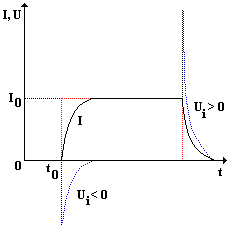
\includegraphics[width=0.3\linewidth]{prechodove_jevy.png}
      \caption{}
  \end{figure}
  \item ZZE platí, to co ztratíme po sepnutí získame po vypnutí -- je to uložené v energii magnetického pole:\\ $E = W = U \cdot I \cdot t = L \cdot \frac{\Delta I}{t} \cdot I \cdot t = L \cdot I \cdot \Delta I = \Phi \cdot \Delta I$ -- mag. tok je přímo úměrný proudu, grafem je zřejmý, energie je plocha pod křivkou, takže energie mag. pole je plocha trojúhelníku $\Rightarrow \Phi \cdot \Delta I = \frac{\Phi \cdot I}{2} = \frac{LI^2}{2}$
\end{itemize}

\subsection{Střídavý proud}
\begin{itemize}
  \item vzniká např. otáčením cívkou v mag. poli (alternátor)
  \item $\Phi = \overrightarrow{B} \cdot \overrightarrow{S} = B \cdot S \cdot \cos \alpha$
  \item $U_i = -\frac{\Delta \Phi}{t} (= -\frac{d \Phi}{dt})$
  \item Okamžitá hodnota: $U = U_m \cdot \sin \omega t$
\end{itemize}
Obvody:
\begin{itemize}
  \item[A)] rezistor zapojený na střídavé napětí:
  \begin{itemize}
    \item platí Ohmův zákon: $i \propto u$
    \item střední hodnota napětí a proudu: $<u> = <i> = 0$
    \item výkon: $p = u \cdot i = U_m \cdot \sin \omega t \cdot I_m \cdot \sin \omega t = U_m \cdot I_m \cdot \sin^2 \omega t = P_m \sin^2 \omega t$
    \item střední hodnota výkonu: $<p> = \frac{P_m}{2}$
    \item Efektivní hodnota: hodnoty takové stejnosměrného proudu/napětí, které kdybychom zapojili tak máme stejný výkon jako střídavý
    $$<p> = P_{STEJNOSM.}$$
    $$\frac{P_m}{2} = P$$
    $$\frac{U_m \cdot I_m}{2} = U \cdot I$$
    $$\frac{RI_m^2}{2} = RI^2$$
    $$\frac{I_m^2}{2} = I^2$$
    $\frac{\sqrt{2}}{2}I_m = I$, $\frac{\sqrt{2}}{2}U_m = U$
    \item takže když se řekne, že je v zásuvce 230V tak to je efektivní napětí -- takže peak napětí je $\sqrt{2} \cdot 230 = 325 V$  CHYBI TADY VSUDE OBRAZKY
  \end{itemize}
  \item[B)] kondenzátor:
  \begin{itemize}
    \item[a)] stejnosměrný proud: žárovka při supštění blikne a pak se vypne -- proud teče jen, dokud se nenabije kondenzátor
    \item[b)] střídavý proud: kondenzátor se střídavě nabíjí a vybíjí a proud jde přes žárovku -- svítí
    \begin{itemize}
      \item napětí: $u = U_m \cdot \sin \omega t$
      \item náboj: $q = C \cdot u = C \cdot U_m \cdot \omega \cdot \cos \omega t =  \frac{U_m}{\frac{1}{\omega C}} \cdot \cos \omega t$
      \item odpor: $\frac{U}{R}$ chybííí
    \end{itemize}
  \end{itemize}

\end{itemize}

nevim nebyl jsem tu jaderná maturita londýn

\begin{itemize}
  \item transformátor, když má sekundární cívka větší počet závitů tak se zvětšuje napětí, transf. nahoru (V nahoru) x dolů
  \item pojistky, jističe
\end{itemize}

\section{Elektromagnetické vlnění}
elmag oscilátor

\part{Optika}
pomoc

\part{Relativita}
nevim neco domyslete si to albert einstein atd.

\section{Relativistická dynamika}

2. NZ.: $F = \frac{\Delta p}{t} = \frac{\Delta \left( m \cdot v \right)}{t} = $ -- při působení konstatntní síly se zvětšuje hybnost. ale rychlost bude vždy $<c \implies$ zvyšuje se hmotnost
$= \frac{\Delta m \cdot v + \Delta v \cdot m}{t} = m \cdot a + \frac{\Delta m \cdot v}{t}$

Odvození m = $f\left(v\right)$
Předpoklady: \begin{enumerate}[1.]
  \item $m = f\left(v\right)$
  \item ZZHybnosti
  \item ZZHmotnosti
\end{enumerate}

Př.: Dokonale nepružná srážka 2 těles se stejnou klidovou hmotností, $v_2 = 0$

\subsection{Kinetická energie}

$E_k = W = \int_{}^{} F dr = \int \frac{dp}{dt} \cdot dr = \int \frac{m \cdot dv + dm \cdot v}{dt} \cdot dr = mc^2 - m_0 c^2$\\
$\implies E = mc^2$ -- celková energie, $E_0 = m_0 c^2$ -- klidová energie\\
$E_k = E - E_0 = mc^2 - m_0 c^2 = m_0 \gamma c^2 - m_0 c^2 = m_0 c^2 (\gamma - 1)$ ($m = \gamma m_0$)\\

Původní vzorec pro kinetickou energii nebyl úplně nepravdivý, je to jenom zanedbání miniaturních členů v této rovnici pro $v \ll c$ (má to smysl asi do $1\% c$)\\

Př.: Urychlíme elektron napětím $1000V$, jakou bude mít rychlost:
\begin{enumerate}[a.]
  \item klasickým vzorcem: $UQ = \frac{1}{2}mv^2 \implies v = \sqrt{\frac{2Ue}{m}} \doteq 0,0625 c = 1,8752 \cdot 10^7 m/s$
  \item spec. teor. rel.: $UQ = m_0 c^2 (\gamma - 1), \gamma = \frac{1}{\sqrt{1-\beta^2}} \implies v = \sqrt{\frac{(\frac{Ue}{m_0 c^2}+1)^2-1}{(\frac{Ue}{m_0 c^2}+1)^2}} \cdot c \doteq 1,8725 \cdot 10^7 m/s$
\end{enumerate}
$\implies$ výsledky stejné na tři platné číslice -- klasický vzorec není naprosto správně, ale je mnohem rychlejší a pro menší rychlosti je úplně dostatečný
\pagebreak

Vraťme se k $E_0 = m_0 c^2$ -- klidová energie
\begin{itemize}
  \item co to ale znamená? $c^2$ jako universální konstanta je jen nějaké číslo, závisející na jednotkové soustavě
  \item hmotnost a energie jsou tedy ekvivalentní, v dobře zvoleném systému jednotek se rovnají
  \item to mi umožňuje počítat hmotnost v Joulech a energii v kilogramech
  \item[$\implies$] hmotnost elektronu: $9,1 \cdot 10^{-31} kg \iff E = mc^2 = 8,19 \cdot 10^{-14} J = 0,511 MeV$
\end{itemize}

\subsection{Záření absolutně černého tělesa}
\begin{itemize}
    \item pohlcuje 100\% dopadajícího záření
    \item pohlcenou energii vyzáří ve formě elmag. záření
    \item modelem třeba komora do které záření vchází malou dutinou a je rozodráženo uvnitř komory
    \item z tohoto experimentálně zjštěny Zákony záření AČT
\end{itemize}

Zákony záření AČT
\begin{itemize}
    \item Kirchhofův: záření závisí jen na teplotě (ne třeba na chem. složení, tlaku, ...)
    \item Planckův: vyzařuje na všech vlnových délkách (tedy není vrchní hranice přes kterou nejde, nebo spodní kterou začíná)
    \begin{center}
        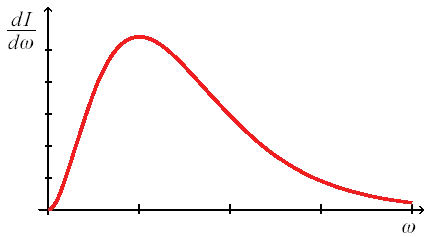
\includegraphics[width=0.5\linewidth]{act.png}
    \end{center}
    \item Wienův: posunovací zákon
    \[
        \lambda_{max} = \frac{b}{T}, b = 2,898 \cdot 10^{-3} m\cdot K
    \]
    \item Stefan-Boltzmannův: $M_e$ -- intenzita vyzařování (plocha pod křivkou)
    \[
        M_e = \sigma \cdot T^4, \sigma 5,67 \cdot 10^{-8} W\cdot m^{-2}\cdot K^{-4}
    \]
\end{itemize}

Pokus o teoretické vysvětlení
\begin{itemize}
    \item zkusíme najít nějakou jinou teorii, která by na to mohla sedět, tak zkuíme třeba termodynamiku -- toto ale vůbec nesedí -- to je tzv. ultrafialová katastrofa
\end{itemize}
\end{document}
